\subsection{Stylized Facts: From Return Dynamics to Market Dependence}
\label{sec:stylized_correlation}

Building on the concepts introduced in Section~\ref{subsec:theory_market_dynamics}, we begin by examining whether the B3 data exhibit the empirical properties commonly observed in financial returns. We first consider the three representative assets defined in Section~\ref{subsec:stylized_method} and then extend the analysis from individual return dynamics to the cross-sectional dependence structure of the broader equity universe. This progression establishes the empirical basis for the spectral decomposition and network analyses that follow.

The selected assets show several familiar return properties: price trajectories differ over the long run, large daily moves cluster in time, and absolute returns remain autocorrelated. Figure~\ref{fig:stylized_facts} brings these complementary diagnostics together for PETR4, VALE3 and BBDC4: normalized prices, daily returns, the complementary cumulative distribution of absolute returns and their autocorrelation \cite{cont_2001_empirical}.

The normalized-price trajectories differ substantially across the three assets, reflecting their distinct long-run dynamics. Their daily returns nevertheless share several common empirical features. Large movements tend to occur in temporally concentrated periods, indicating volatility clustering, while the complementary cumulative distributions show that large absolute returns occur more frequently than expected under a Gaussian benchmark. The autocorrelation of absolute returns remains positive over several lags, providing further evidence of persistent volatility \cite{cont_2001_empirical}.

Table~\ref{tab:descriptive_stats} quantifies the same diagnostics. All three series have means close to zero, substantial kurtosis and non-negligible counts of large absolute returns. PETR4 has the largest negative daily observation in the 2006--2025 window, while VALE3 and BBDC4 also show stress-period extremes. The autocorrelations of absolute returns remain positive across several lags, especially for VALE3.

\begin{center}
\captionof{table}{Descriptive statistics for the three demonstration assets, 2006--2025.}
\label{tab:descriptive_stats}
\scriptsize
\setlength{\tabcolsep}{2.8pt}
\resizebox{\linewidth}{!}{%
\begin{tabular}{lrrrrrrrrrrrrrrr}
\toprule
Symbol & $n$ & Mean & Std. & Skew. & Ex. kurt. & Min. & Max. &
VaR$_{1\%}$ & VaR$_{5\%}$ &
$|r|>10\%$ & $|r|>20\%$ &
ACF$_1$ & ACF$_5$ & ACF$_{20}$ & ACF$_{60}$ \\
\midrule
BBDC4 & 4953 & 0.0003 & 0.0218 &  0.02 &  7.96 & -0.1910 & 0.1999 & -0.0559 & -0.0312 & 16 & 0 & 0.207 & 0.174 & 0.122 & 0.044 \\
PETR4 & 4953 & 0.0004 & 0.0276 & -0.76 & 11.55 & -0.3524 & 0.2007 & -0.0767 & -0.0408 & 41 & 4 & 0.254 & 0.209 & 0.140 & 0.062 \\
VALE3 & 4953 & 0.0005 & 0.0258 & -0.22 &  7.51 & -0.2814 & 0.1936 & -0.0676 & -0.0381 & 26 & 2 & 0.231 & 0.207 & 0.169 & 0.119 \\
\bottomrule
\end{tabular}}
\end{center}

\noindent\footnotesize\emph{Notes:} Mean, Std., extrema and VaR are reported to four decimal places; skewness and excess kurtosis to two; autocorrelations to three; and event counts as integers. Mean and Std. are computed from daily log returns. VaR$_{1\%}$ and VaR$_{5\%}$ are empirical lower-tail return quantiles, and ACF$_\ell$ is the autocorrelation of absolute returns at lag $\ell$ trading days.

\begin{center}
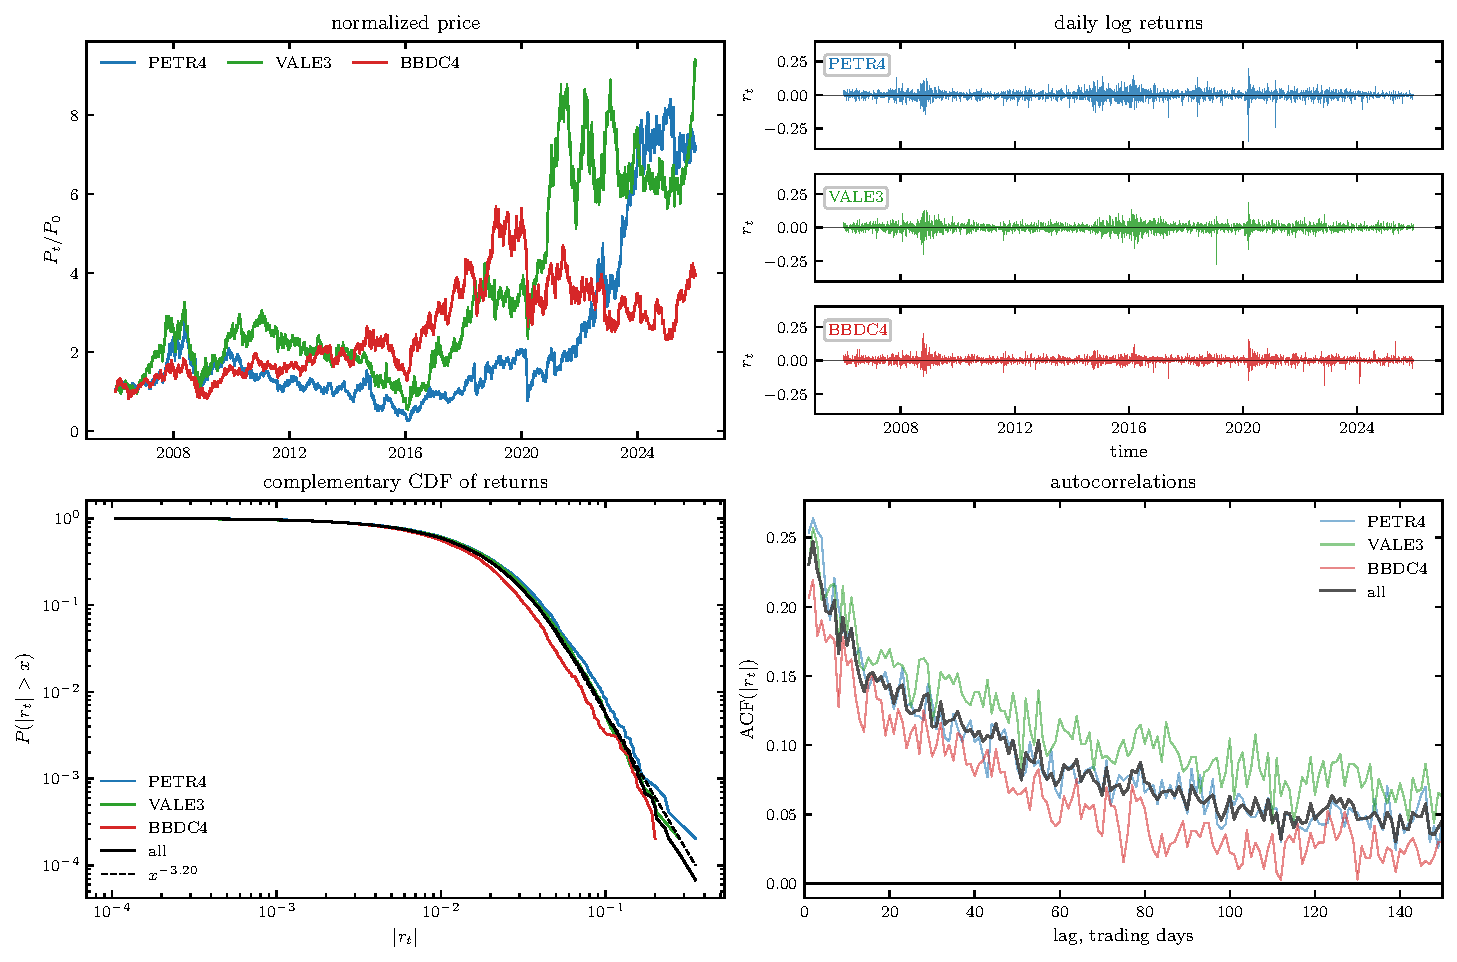
\includegraphics[width=0.95\linewidth]{images/figure_1d_stylized_facts_demo_assets_clean_2006_2025.pdf}
\captionof{figure}{Stylized facts for PETR4, VALE3 and BBDC4 over 2006--2025. The panels show normalized prices, daily log returns, the complementary cumulative distribution of absolute returns and autocorrelations of absolute returns. The return panel uses three vertically aligned subpanels with a common scale and a zero reference line for each asset.}
\label{fig:stylized_facts}
\end{center}

\normalsize

Taken together, the visual and numerical evidence shows that the selected B3 assets exhibit well-known empirical regularities of financial returns, including non-Gaussian behavior and volatility persistence. This motivates extending the analysis from individual return dynamics to the dependence structure across the broader equity universe.

We now turn from individual return behaviour to cross-sectional dependence. The core historical universe contains 58 assets, producing $N(N-1)/2=1653$ unique asset pairs. The static summaries use the available overlap for each pair and therefore retain the broader unbalanced historical coverage. The subsequent RMT analysis instead uses the complete synchronized 58-asset panel from 23 August 2006 to 15 August 2024. This distinction ensures that the descriptive correlation evidence is not confused with the common-sample correlation matrix used for the spectral decomposition. 

The pairwise correlations are positive on average but dispersed, and within-sector pairs tend to be more strongly related than pairs from different sectors. Figure~\ref{fig:correlation_structure} shows both the full distribution and the within-sector versus between-sector comparison. Across the broader unbalanced pair coverage, the mean is close to 0.24 and the median close to 0.23. This level of average dependence suggests the presence of a common component, but the distribution remains dispersed. The dispersion is important because it leaves room for sectoral and subsectoral organization instead of a single homogeneous market block.

The sectoral comparison provides a first indication that this heterogeneity is economically structured. Within-sector correlations are shifted toward higher values relative to between-sector correlations. As summarized in Table~\ref{tab:sector_corr_summary}, the mean within-sector correlation is 0.3433, compared with 0.2249 for between-sector pairs, producing a difference of $\Delta_{\mathrm{sector}}=0.1184$.

\begin{center}
\begin{minipage}{0.5\linewidth}
  \centering
  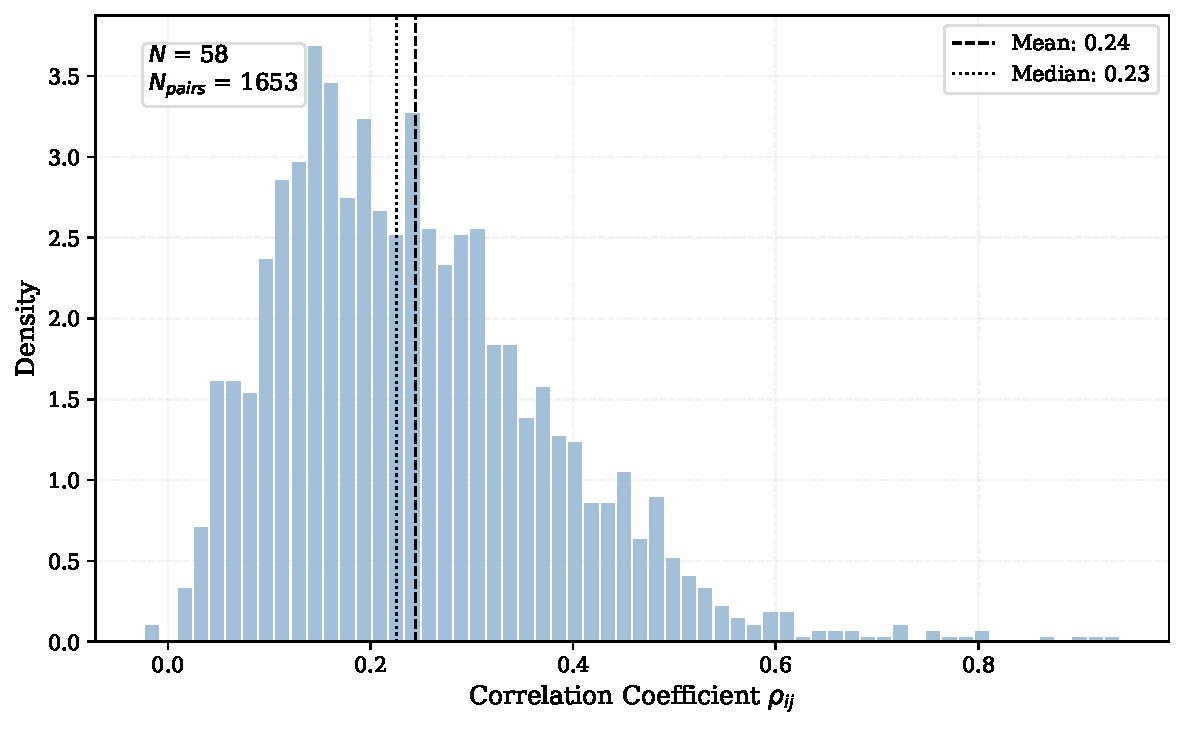
\includegraphics[width=\linewidth]{images/figure_2_correlation_histogram.pdf}
  \vspace{0.2cm}

  \small (a) Full pairwise distribution.
\end{minipage}
\hfill
\begin{minipage}{0.48\linewidth}
  \centering
  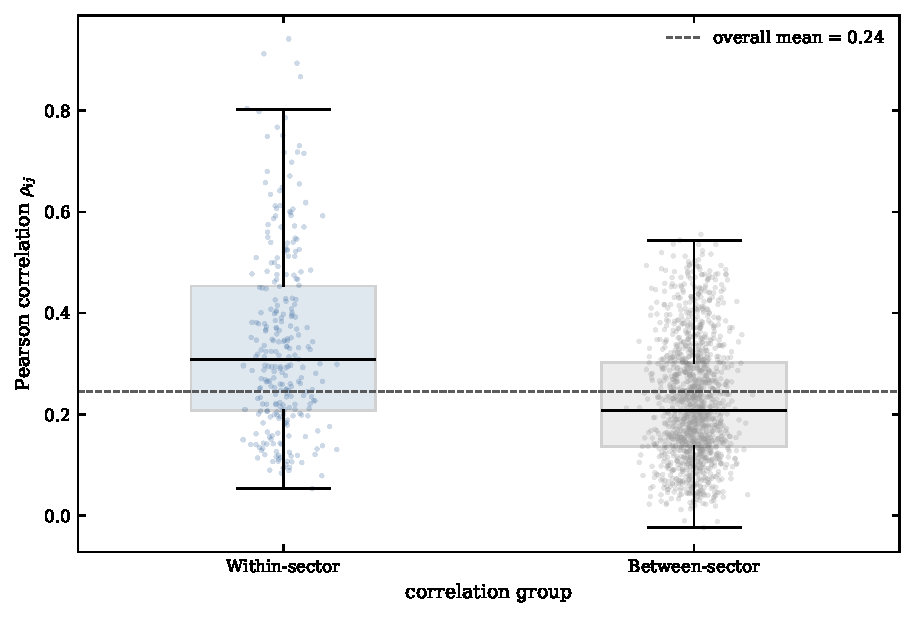
\includegraphics[width=\linewidth]{images/figure_3_sector_correlation_distribution.pdf}
  \vspace{0.2cm}

  \small (b) Within-sector and between-sector pairs.
\end{minipage}

\captionof{figure}{Correlation structure in the core historical universe. Panel (a) shows the full Pearson correlation distribution. Panel (b) compares within-sector and between-sector correlations using the initial macro-sector classification.}
\label{fig:correlation_structure}
\end{center}

\begin{center}
\captionof{table}{Within-sector and between-sector correlation summary.}
\label{tab:sector_corr_summary}
\begin{tabular}{lrrrrrr}
\toprule
Group & Pairs & Mean & Median & Std. dev. & Min & Max \\
\midrule
Within-sector & 275 & 0.3433 & 0.3082 & 0.1819 & 0.0534 & 0.9402 \\
Between-sector & 1378 & 0.2249 & 0.2076 & 0.1166 & -0.0236 & 0.5552 \\
\bottomrule
\end{tabular}
\end{center}


The difference is economically meaningful. Within-sector pairs have mean correlation 0.3433, while between-sector pairs have mean correlation 0.2249, giving $\Delta_{\mathrm{sector}}=0.1184$. An asset-level label-permutation test with 10,000 sector-label reallocations preserves both the observed dependency matrix and the sector-size vector, without treating overlapping pairs as independent observations. None of the permuted statistics reaches the observed difference (null 95th percentile $=0.0245$; one-sided Monte Carlo $p\approx 10^{-4}$, the minimum attainable at this simulation count). The observed difference is also supported by the sector-label permutation analysis reported later in the robustness assessment. At this stage, the relevant result is that the dependency matrix is not characterized solely by homogeneous positive co-movement: stronger relationships are also concentrated within the economic grouping used in the analysis.

The static correlation distribution, however, does not show whether these relationships remain stable through time. We therefore examine selected economically interpretable asset pairs under different dynamic correlation estimators. Figure~\ref{fig:dynamic_pairwise} includes PETR4--VALE3, representing two large commodity-exposed firms in distinct subsectors; BBDC4--BBAS3 in financials; GGBR4--USIM5 in steel and metallurgy; and ELET3--CMIG4 in utilities. These pairs are illustrative rather than intended to represent all possible pairwise relationships.

The pairwise estimates show that individual dependencies can strengthen, weaken, or temporarily break down over time. The 20-day Pearson estimates respond rapidly to local variation, whereas the 60-day estimates provide smoother representations of persistent relationships. The EWMA estimates provide an intermediate view by assigning greater weight to recent observations. The common conclusion across these estimators is that a single full-sample correlation should be interpreted as a long-run summary of an underlying time-varying relationship.

We finally move from individual pairs to market-wide synchronization. Figure~\ref{fig:rolling_corr} reports the average pairwise market correlation estimated with 252- and 504-trading-day rolling windows. Because historical coverage changes in the earliest part of the sample, each window uses the assets available during that period, ranging from approximately 40 assets initially to the complete 58-asset universe in later years. The series should therefore be interpreted as a descriptive measure of average available cross-sectional dependence.

Market-wide correlation varies through time and increases around the 2008 global financial crisis and the 2020 COVID-19 shock. Figure~\ref{fig:rolling_corr} remains close to 0.2 during 2015--2016, so that interval does not show a comparable increase in this measure. These episodes show that the positive dependence observed in the static correlation distribution is not constant through time.

Taken together, the results reveal three complementary features of the B3 dependency structure: positive but heterogeneous cross-sectional correlations, stronger dependence within economic sectors, and substantial variation in synchronization over time. The presence of broad co-movement alongside more localized relationships raises the next question in the empirical sequence: how much of the observed correlation structure is associated with a dominant collective market mode, how much remains in smaller group-level components, and how much is compatible with sampling noise? We address this question next through Random Matrix Theory.

\begin{center}
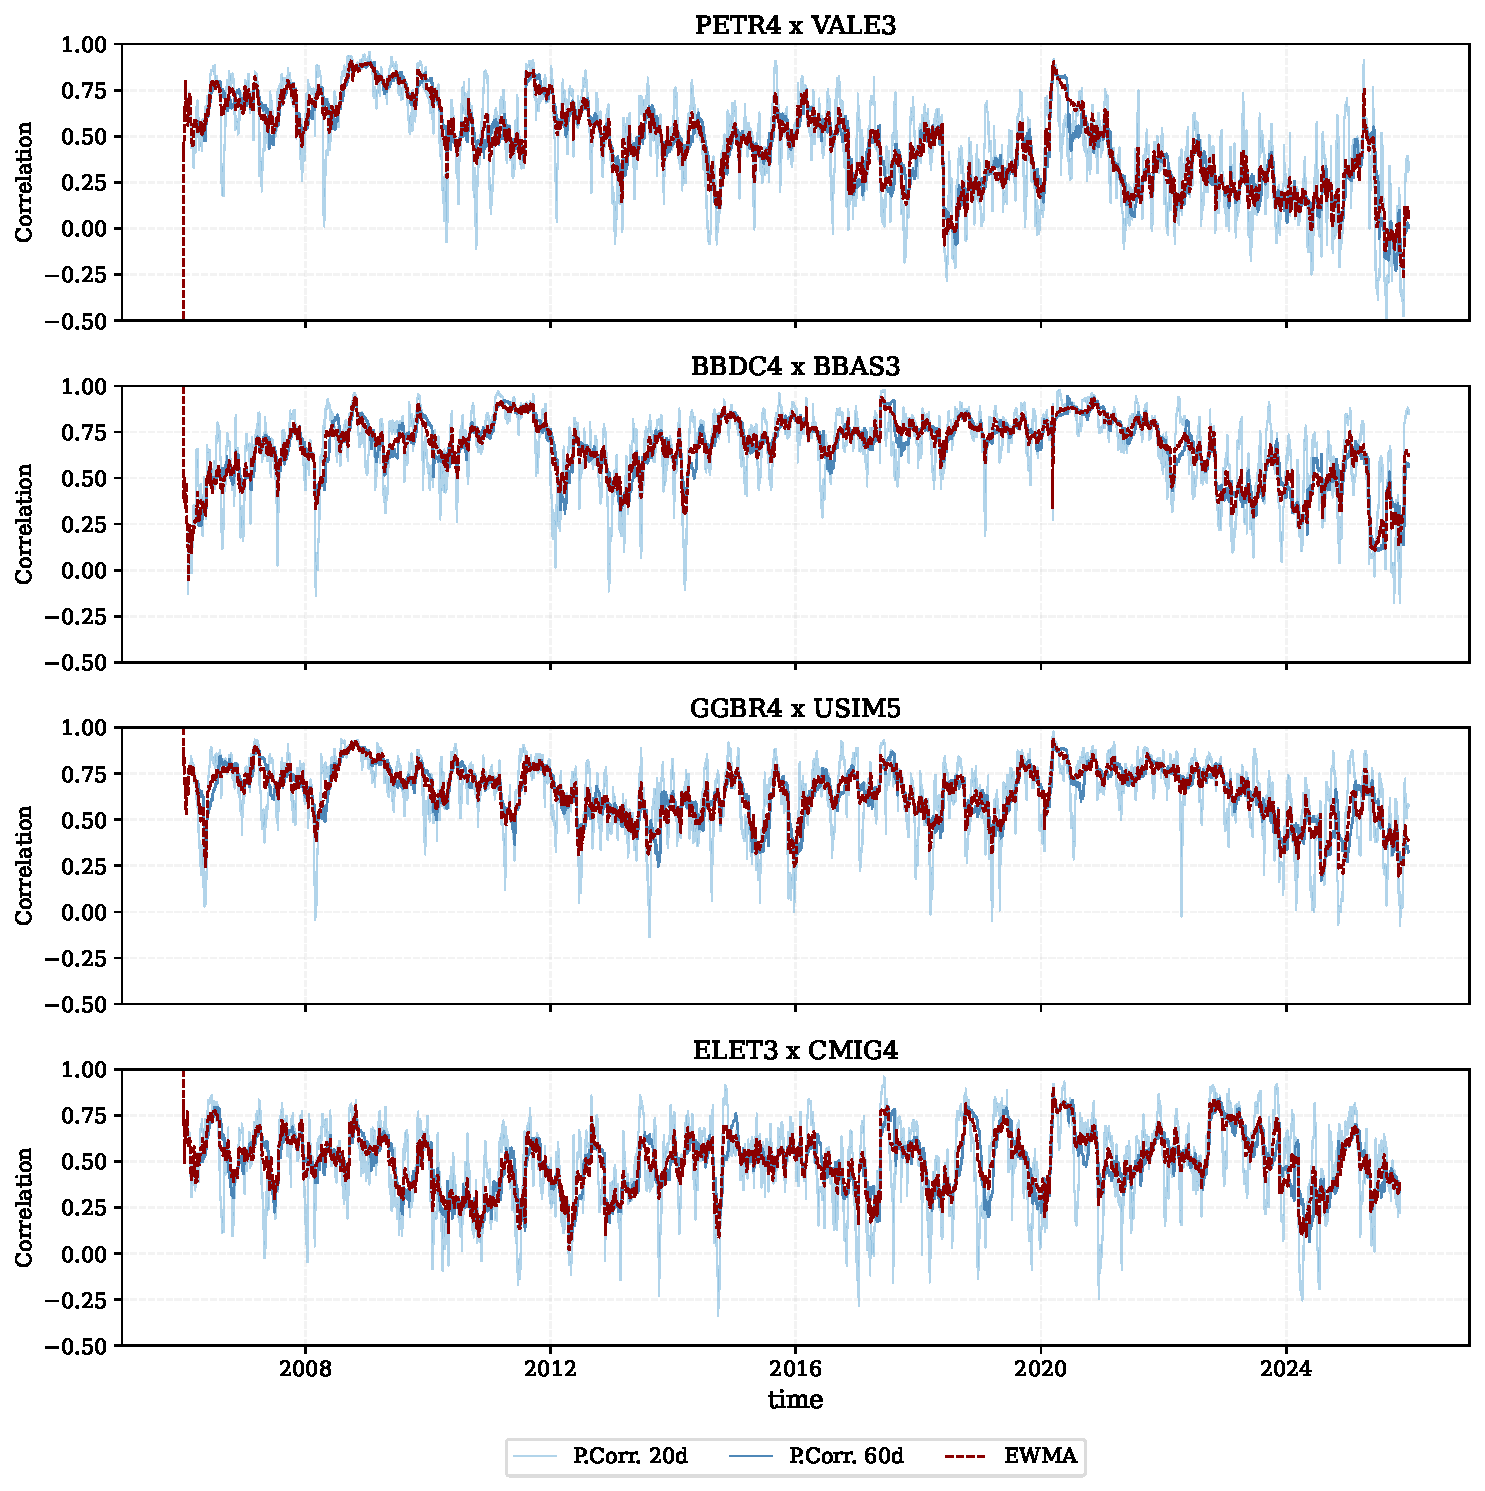
\includegraphics[width=\linewidth]{images/figure_5_dynamic_pairwise_correlations.pdf}
\captionof{figure}{Dynamic pairwise correlations for selected economically interpretable asset pairs. Pearson estimates use 20- and 60-trading-day windows; EWMA uses a 20-day half-life. The estimates show how individual dependencies can vary across time scales.}
\label{fig:dynamic_pairwise}
\end{center}


\begin{center}
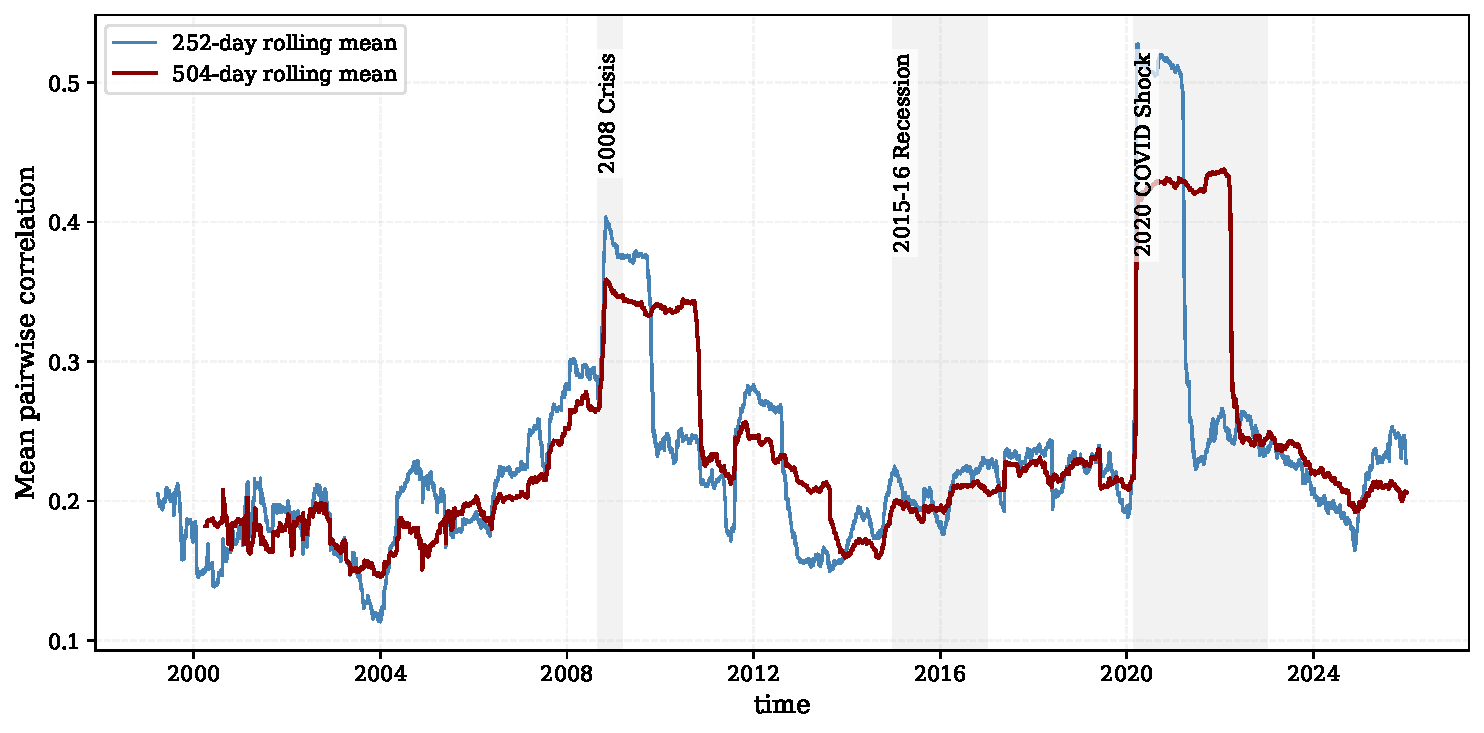
\includegraphics[width=0.95\linewidth]{images/figure_4_rolling_average_correlation.pdf}
\captionof{figure}{Rolling average market correlation for the core historical universe, estimated with 252- and 504-trading-day windows. Each window uses the assets available during that period.}
\label{fig:rolling_corr}
\end{center}
